\section{再论仿射簇}\label{sec:affine-varieties-revisited}

本节的主要目标是证明, 若 $X_{0}\subseteq\mathbb{A}^{n}$ 为仿射簇, 则 $X_{0}$ 上的多项式函数与典范对应的拟射影簇 $j_{0}(X_{0})$ 上的正则函数相同. 证明该断言的关键困难在于, 正则函数只须局部由多项式的商给出, 多项式函数却必须在整体上表示为一个多项式的限制. 尽管多项式函数看上去比正则函数受限得多, 下面的结果表明, 这两种看似不同的描述在仿射簇上给出完全相同的函数集合.

\begin{Theorem}{仿射簇上的正则函数是多项式函数}\leavevmode\label{thm:regular-functions-on-affine-varieties-are-polynomial}
设 $X_{0}\subseteq\mathbb{A}^{n}$ 为仿射簇, $X=j_{0}(X_{0})\subseteq\mathbb{P}^{n}$ 为相应的拟射影簇. 则 $X$ 的正则函数环与 $X_{0}$ 的坐标环之间有典范同构
\[
  K[X]=K[X_{0}],
\]
它将 $F\in K[X]$ 送到 $F_{0}=F\circ j_{0}\in K[X_{0}]$.
\end{Theorem}
\begin{Proof}
设 $F:X\to K$ 为正则函数, 令 $F_{0}=F\circ j_{0}:X_{0}\to K$, 从而
\[
  F_{0}(a_{1},\ldots,a_{n})=F([1:a_{1}:\cdots:a_{n}]).
\]
证明中最困难的部分是说明 $F_{0}$ 实际上是 $X_{0}$ 上的多项式函数, 因而是坐标环的元素. 应用正则函数的定义, 再令 $x_{0}=1$, 可知对任意 $p\in X_{0}$, 都能选取多项式 $f_{p},g_{p}\in K[x_{1},\ldots,x_{n}]$, 使 $g_{p}(p)\ne0$, 且
\[
  F_{0}(a)=\frac{f_{p}(a)}{g_{p}(a)}
  \qquad\text{对所有 }a\in X_{0}\setminus\mathcal{V}_{\mathbb{A}}(g_{p}).
\]
此外, 可以假设 $f_{p},g_{p}$ 都在 $X_{0}$ 的每个不含 $p$ 的不可约分支 $Z$ 上消没. 若它们未在 $Z$ 上消没, 可以将 $f_{p}$ 和 $g_{p}$ 同时乘以一个在整个 $Z$ 上消没而不在 $p$ 消没的多项式. 对每个 $p\in X_{0}$, 选取一对这样的 $(f_{p},g_{p})$.

我们断言, 对任意 $p,q\in X_{0}$, 多项式 $f_{p}g_{q}$ 和 $f_{q}g_{p}$ 定义同一个函数 $X_{0}\to K$. 为此, 证明它们在每个不可约分支 $Z\subseteq X_{0}$ 上相等. 若 $p\notin Z$ 或 $q\notin Z$, 假设蕴含 $f_{p}g_{q}=f_{q}g_{p}=0$ 在 $Z$ 上成立. 另一方面, 若 $p,q\in Z$, 则等式
\[
  \frac{f_{p}(a)}{g_{p}(a)}=F_{0}(a)=\frac{f_{q}(a)}{g_{q}(a)}
\]
对所有使 $g_{p}$ 和 $g_{q}$ 都不消没的 $a$ 成立. 这意味着多项式函数 $f_{p}g_{q}$ 和 $f_{q}g_{p}$ 在 $Z\setminus\mathcal{V}_{\mathbb{A}}(g_{p}g_{q})$ 上相等, 后者是不可约簇 $Z$ 的一个非空开集. 由 Proposition~\ref{prop:nonempty-open-in-irreducible-space-is-dense}, $Z\setminus\mathcal{V}_{\mathbb{A}}(g_{p}g_{q})$ 在 $Z$ 中稠密, 从而 (见 Exercise~\ref{ex:affine-closure-preserves-vanishing-ideal}) $f_{p}g_{q}$ 和 $f_{q}g_{p}$ 在整个 $Z$ 上相等, 证得上述断言.

现在定义由 $F_{0}$ 所选的全部局部表达式的分母生成的理想
\[
  J=\langle g_{p}\mid p\in X_{0}\rangle\subseteq K[x_{1},\ldots,x_{n}].
\]
由于 $J$ 的每个生成元都在 $X_{0}$ 的某点处不消没, 有
\[
  \mathcal{V}_{\mathbb{A}}(J+\mathcal{I}_{\mathbb{A}}(X_{0}))
   =\mathcal{V}_{\mathbb{A}}(J)\cap X_{0}=\varnothing,
\]
由零点定理得 $J+\mathcal{I}_{\mathbb{A}}(X_{0})=K[x_{1},\ldots,x_{n}]$. 特别地, 这意味着 $1\in J+\mathcal{I}_{\mathbb{A}}(X_{0})$, 所以可以写
\begin{equation}\label{eq:local-denominators-generate-unit-modulo-affine-ideal}
  1=h_{1}g_{p_{1}}+\cdots+h_{k}g_{p_{k}}+f,
\end{equation}
其中 $p_{1},\ldots,p_{k}\in X_{0}$, $h_{1},\ldots,h_{k}\in K[x_{1},\ldots,x_{n}]$, 且 $f\in\mathcal{I}_{\mathbb{A}}(X_{0})$.

现在断言, 对每个 $a\in X_{0}$, 都有
\[
  F_{0}(a)=h_{1}(a)f_{p_{1}}(a)+\cdots+h_{k}(a)f_{p_{k}}(a).
\]
为此, 令 $a\in X_{0}$. 由 \eqref{eq:local-denominators-generate-unit-modulo-affine-ideal}, 对某个 $i$ 有 $g_{p_{i}}(a)\ne0$; 不妨假设 $g_{p_{1}}(a)\ne0$. 则
\[
  \begin{aligned}
  F_{0}(a)&=\frac{f_{p_{1}}(a)}{g_{p_{1}}(a)}\\
    &=\left(\sum_{i=1}^{k}h_{i}(a)g_{p_{i}}(a)\right)\frac{f_{p_{1}}(a)}{g_{p_{1}}(a)}\\
    &=\sum_{i=1}^{k}h_{i}(a)\frac{f_{p_{i}}(a)g_{p_{1}}(a)}{g_{p_{1}}(a)}\\
    &=\sum_{i=1}^{k}h_{i}(a)f_{p_{i}}(a),
  \end{aligned}
\]
其中第二个等式用到方程 \eqref{eq:local-denominators-generate-unit-modulo-affine-ideal}, 第三个等式用到 $f_{p_{1}}g_{p_{i}}=f_{p_{i}}g_{p_{1}}$ 作为 $X_{0}$ 上的函数成立这一事实. 这就证明了 $F_{0}$ 在 $X_{0}$ 上可以由多项式函数 $F_{0}=[h_{1}f_{p_{1}}+\cdots+h_{k}f_{p_{k}}]\in K[X_{0}]$ 整体地实现.

特别地, 现在知道 $F\mapsto F_{0}$ 确定了一个函数 $K[X]\to K[X_{0}]$, 显然是 $K$-代数同态. 此外, 它是双射. 若 $F_{0}\in K[X_{0}]$ 是 $X_{0}$ 上的多项式函数, 可以选取代表 $F_{0}=[f_{0}]$, 其中 $f_{0}\in K[x_{1},\ldots,x_{n}]$, 将它齐次化成某个 $d$ 次的齐次多项式 $f\in K[x_{0},x_{1},\ldots,x_{n}]$. 再令 $F=f/x_{0}^{d}$, 得到 $X$ 上的一个正则函数, 其去齐次化为 $F_{0}$. 因此映射 $K[X]\to K[X_{0}]$ 是 $K$-代数同构, 如所需.
\end{Proof}

有了 Theorem~\ref{thm:regular-functions-on-affine-varieties-are-polynomial}, 就可以计算任何由仿射簇的自然嵌入得到的拟射影簇的正则函数环. 下面的例子展示如何对上一节遇到的一个特定拟射影簇作此计算.

\begin{Example}{$\mathcal{V}(w^{2}-xy)\setminus\mathcal{V}(w)$ 上的正则函数环}\leavevmode\label{ex:regular-function-ring-of-punctured-projective-conic}
考察拟射影簇
\[
  Y=\mathcal{V}(w^{2}-xy)\setminus\mathcal{V}(w)\subseteq\mathbb{P}^{2},
\]
可以把它与 $j_{0}(Y_{0})$ 等同, 其中
\[
  Y_{0}=\mathcal{V}_{\mathbb{A}}(1-xy)\subseteq\mathbb{A}^{2}.
\]
由 Theorem~\ref{thm:regular-functions-on-affine-varieties-are-polynomial}, 有
\[
  K[Y]=K[Y_{0}]
   =\frac{K[x,y]}{\mathcal{I}_{\mathbb{A}}(Y_{0})}
   =\frac{K[x,y]}{\langle1-xy\rangle}=K[x,x^{-1}].
\]
\end{Example}

现在已经知道, 仿射簇上的多项式函数与其对应的拟射影簇上的正则函数一致. 再稍作论证, 就可以证明多项式映射和正则映射也一样.

\begin{Corollary}{仿射簇之间的正则映射是多项式映射}\leavevmode\label{cor:regular-maps-between-affine-varieties-are-polynomial}
设 $X_{0}\subseteq\mathbb{A}^{m}$ 和 $Y_{0}\subseteq\mathbb{A}^{n}$ 为仿射簇, $X=j_{0}(X_{0})\subseteq\mathbb{P}^{m}$ 和 $Y=j_{0}(Y_{0})\subseteq\mathbb{P}^{n}$ 为相应的拟射影簇. 将 $F:X\to Y$ 送到 $F_{0}=j_{0}^{-1}\circ F\circ j_{0}$, 给出双射
\[
  \left\{\begin{gathered}\text{正则映射}\\ X\to Y\end{gathered}\right\}
   \longrightarrow
  \left\{\begin{gathered}\text{多项式映射}\\ X_{0}\to Y_{0}\end{gathered}\right\}.
\]
\end{Corollary}
\begin{Proof}
若 $F:X\to Y$ 为正则映射, 则由正则映射和正则函数的定义, 复合映射 $j_{0}^{-1}\circ F:X\to Y_{0}\subseteq\mathbb{A}^{n}$ 由下式给出:
\[
  (j_{0}^{-1}\circ F)(a)=(\widetilde{F}_{1}(a),\ldots,\widetilde{F}_{n}(a)),
\]
其中每个 $\widetilde{F}_{i}:X\to K$ 都是 $X$ 上的正则函数. 于是由 Theorem~\ref{thm:regular-functions-on-affine-varieties-are-polynomial} 可知
\[
  \widetilde{F}_{1}\circ j_{0},\ldots,\widetilde{F}_{n}\circ j_{0}\in K[X_{0}].
\]
特别地, 它们每个都是 $X_{0}$ 上的多项式函数. 因此
\[
  (j_{0}^{-1}\circ F\circ j_{0})(a)
   =((\widetilde{F}_{1}\circ j_{0})(a),\ldots,(\widetilde{F}_{n}\circ j_{0})(a))
\]
是多项式映射 $X_{0}\to Y_{0}$. 这说明对应 $F\mapsto F_{0}$ 确实把正则映射送到多项式映射. 稍加思考可知, 它实际上是双射 (见 Exercise~\ref{ex:affine-polynomial-map-correspondence-is-bijective}).
\end{Proof}

至此, 与第~\ref{sec:quasiprojective-regular-maps-and-functions}~节关于射影簇的讨论平行, 我们已经证明仿射簇范畴嵌入拟射影簇范畴. 不过, 这种情形有一个明显的不足: 尽管每个仿射簇都可自然地与一个拟射影簇等同, 以此方式得到的拟射影簇这一类别在同构下并不保持. 下一例说明这一现象.

\begin{Example}{$\mathbb{A}^{1}\setminus\{0\}$ 同构于 $\mathcal{V}(1-xy)\subseteq\mathbb{A}^{2}$}\leavevmode\label{ex:punctured-affine-line-isomorphic-to-hyperbola}
\BookPairedFigure{
令 $X_{0}=\mathbb{A}^{1}\setminus\{0\}$. 作为 $\mathbb{A}^{1}$ 的子集, $X_{0}$ 不是仿射簇; 实际上, $\mathbb{A}^{1}$ 的真仿射簇只有有限点集. 不过, 可以把 $X_{0}$ 与拟射影簇
\[
  X=j_{0}(X_{0})=\mathbb{P}^{1}\setminus\mathcal{V}(xy)
\]
自然等同. 我们在 Example~\ref{ex:isomorphism-of-punctured-projective-line-and-conic} 中看到, $X$ 同构于拟射影簇
\[
  Y=\mathcal{V}(w^{2}-xy)\setminus\mathcal{V}(w)\subseteq\mathbb{P}^{2},
\]
而此拟射影簇确实自然地与一个仿射簇等同:
\[
  Y=j_{0}(Y_{0})\quad\text{其中}\quad
  Y_{0}=\mathcal{V}(1-xy)\subseteq\mathbb{A}^{2}.
\]
}{
\phantomsection\label{fig:affine-hyperbola-punctured-line-isomorphism}%
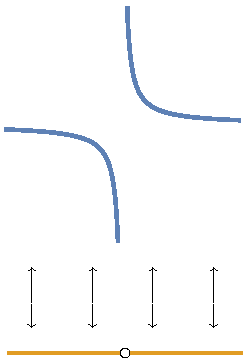
\includegraphics[width=\linewidth]{figures/affine-hyperbola-punctured-line-isomorphism.pdf}
}
因此, 即使 $X$ 并非自然地来自仿射簇, 它仍同构于一个自然来自仿射簇的拟射影簇. 上图描绘的是 $Y_{0}=\mathcal{V}(1-xy)\subseteq\mathbb{A}^{2}$ 与 $X_{0}=\mathbb{A}^{1}\setminus\{0\}\subseteq\mathbb{A}^{1}$ 之间的拟射影同构.
\end{Example}

由于通常希望簇的性质在同构下保持, 这一例子表明我们的术语陷入一种不理想的境地. 我们用一种直接的办法解决它: 只需修改\textquotedbl{}仿射簇\textquotedbl{}的定义, 要求它在拟射影簇的同构下保持不变.

\begin{Definition}{仿射簇}\leavevmode\label{def:affine-variety-as-quasiprojective-variety}
若拟射影簇 $X\subseteq\mathbb{P}^{m}$ 同构于某个拟射影簇 $Y\subseteq\mathbb{P}^{n}$, 且对某个 Zariski 闭子集 $Y_{0}\subseteq\mathbb{A}^{n}$ 有 $Y=j_{0}(Y_{0})$, 就称 $X$ 为\emph{仿射簇}.
\end{Definition}

尽管 Example~\ref{ex:punctured-affine-line-isomorphic-to-hyperbola} 中的拟射影簇 $\mathbb{P}^{1}\setminus\mathcal{V}(xy)$ 不\emph{等于}任何 Zariski 闭子集 $X_{0}\subseteq\mathbb{A}^{1}$ 的 $j_{0}(X_{0})$, 我们已经验证, $\mathbb{P}^{1}\setminus\mathcal{V}(xy)$ \emph{同构于}一个拟射影簇 $Y\subseteq\mathbb{P}^{2}$, 使对某个 Zariski 闭子集 $Y_{0}\subseteq\mathbb{A}^{2}$ 有 $Y=j_{0}(Y_{0})$. 因此根据 Definition~\ref{def:affine-variety-as-quasiprojective-variety}, 以下把拟射影簇 $\mathbb{P}^{1}\setminus\mathcal{V}(xy)$ 称为仿射簇.

这一术语却又引出了新的问题: 现在\textquotedbl{}仿射簇\textquotedbl{}指特定类型的拟射影簇, 那么原先称作仿射簇的对象, 即作为一族多项式的消没集而得到的 $\mathbb{A}^{n}$ 的子集, 应怎样称呼? 和上一段一样, 以下用 Zariski 拓扑的语言称呼它们.

\begin{BookTerminologyChange}\leavevmode\label{def:affine-vanishing-sets-are-called-zariski-closed-subsets}
对某个子集 $S\subseteq K[x_{1},\ldots,x_{n}]$, 形如 $\mathcal{V}_{\mathbb{A}}(S)$ 的 $\mathbb{A}^{n}$ 的子集, 以下称为 $\mathbb{A}^{n}$ 的 \emph{(Zariski) 闭子集}.
\end{BookTerminologyChange}

\BookPairedNote{
因此, 尽管 $\mathbb{A}^{1}\setminus\{0\}$ 不是 $\mathbb{A}^{1}$ 的 Zariski 闭子集, 从而按本书先前的术语不是仿射簇, 现在却可以称它为仿射簇, 因为根据 Definition~\ref{def:affine-variety-as-quasiprojective-variety}, 它作为拟射影簇是仿射的.
}{
注意, 这里已经开始不再区分子集 $X\subseteq\mathbb{A}^{n}$ 与相应的子集 $j_{0}(X)\subseteq\mathbb{P}^{n}$. 读者会逐渐习惯这种轻微的记号滥用.
}
这个具体例子是下一节将证明的一般结果的特例: 闭集 $X\subseteq\mathbb{A}^{n}$ 中使单个多项式不消没的点构成的子集, 总是仿射簇.

读者可能会问, 关于射影簇是否也需要类似的术语变更. 实际上, 在射影情形不需要, 因为射影簇已经在同构下保持. 更准确地说, 由本章稍后的讨论可知, 若 $X\subseteq\mathbb{P}^{m}$ 和 $Y\subseteq\mathbb{P}^{n}$ 为同构的拟射影簇, 则其中一个在其环境射影空间中 Zariski 闭当且仅当另一个也 Zariski 闭 (Corollary~\ref{cor:projectivity-invariant-under-quasiprojective-isomorphism}).

与此同时, 本节的最后一个目标是给出仿射空间中一个可以证明不是仿射簇的拟射影簇的例子.

\begin{Example}{$\mathbb{A}^{2}\setminus\{(0,0)\}$ 不是仿射簇}\leavevmode\label{ex:punctured-affine-plane-is-not-affine}
考察 $X_{0}=\mathbb{A}^{2}\setminus\{(0,0)\}$. 将它与拟射影簇 (Exercise~\ref{ex:punctured-affine-plane-as-projective-open-and-its-function-ring})
\[
  X=\mathbb{P}^{2}\setminus\mathcal{V}(x_{0}x_{1},x_{0}x_{2})
\]
等同. 反设 $X$ 是仿射簇, 则存在同构 $F:Y\to X$, 其中对某个闭子集 $Y_{0}\subseteq\mathbb{A}^{n}$ 有 $Y=j_{0}(Y_{0})$.

考察 $K[X]$ 中的正则函数 $G_{1}=x_{1}/x_{0}$ 和 $G_{2}=x_{2}/x_{0}$. 注意 $X$ 上不存在使 $G_{1}$ 和 $G_{2}$ 同时消没的点. 因此, $F^{*}G_{1}$ 和 $F^{*}G_{2}$ 在 $Y$ 上也没有共同的消没点. 由于 $K[Y]=K[Y_{0}]$ (Theorem~\ref{thm:regular-functions-on-affine-varieties-are-polynomial}), 对闭集 $Y_{0}\subseteq\mathbb{A}^{n}$ 应用零点定理得到 $K[Y]=\langle F^{*}G_{1},F^{*}G_{2}\rangle$ (见 Exercise~\ref{ex:regular-functions-with-no-common-zero-generate-unit}). 但是, 因为 $F^{*}:K[X]\to K[Y]$ 是同构 (Proposition~\ref{prop:quasiprojective-isomorphism-induces-regular-function-ring-isomorphism}), 可推出 $K[X]=\langle G_{1},G_{2}\rangle$.

另一方面, Lemma~\ref{lem:regular-functions-on-projective-open-subsets-are-global-quotients} 蕴含 (Exercise~\ref{ex:punctured-affine-plane-as-projective-open-and-its-function-ring})
\[
  K[X]\cong K[x_{1},x_{2}].
\]
理想 $\langle G_{1},G_{2}\rangle$ 在此同构下对应于 $\langle x_{1},x_{2}\rangle\subseteq K[x_{1},x_{2}]$, 因而为真理想, 与 $\langle G_{1},G_{2}\rangle=K[X]$ 矛盾. 这一矛盾意味着 $X$ 不可能是仿射簇.
\end{Example}

\BookExerciseHeading
\begin{BookExercises}
  \item\label{ex:laurent-polynomial-on-projective-conic-as-homogeneous-quotient} 令 $Y=\mathcal{V}(w^{2}-xy)\subseteq\mathbb{P}^{2}$, 如 Example~\ref{ex:regular-function-ring-of-punctured-projective-conic} 所示, 在那里已经看到
  \[
    K[Y]=K[x,x^{-1}].
  \]
  把与 $x^{4}-3x^{-1}\in K[x,x^{-1}]$ 对应的正则函数 $Y\to K$ 描述为 $K[w,x,y]$ 中同次数的齐次多项式的商.
  \item\label{ex:homogenize-polynomial-map-between-affine-curves-and-surfaces} 令 $X_{0}=\mathcal{V}_{\mathbb{A}}(x_{2}-x_{1}^{2})\subseteq\mathbb{A}^{2}$, $Y_{0}=\mathcal{V}_{\mathbb{A}}(y_{1}y_{2}-y_{3})\subseteq\mathbb{A}^{3}$. 考察如下给出的多项式映射 $X_{0}\to Y_{0}$:
  \[
    (a_{1},a_{2})\mapsto(a_{1}-a_{1}^{2},a_{1}+a_{2},a_{1}^{2}-a_{2}^{2}).
  \]
  用同次数的齐次多项式描述相应的拟射影簇之间的正则映射 $X\to Y$, 其中 $X=j_{0}(X_{0})\subseteq\mathbb{P}^{2}$ 且 $Y=j_{0}(Y_{0})\subseteq\mathbb{P}^{3}$.
  \item\label{ex:affine-polynomial-map-correspondence-is-bijective} 推广上一题中的构造, 证明 Corollary~\ref{cor:regular-maps-between-affine-varieties-are-polynomial} 陈述中的对应可逆, 因而是双射.
  \item\label{ex:punctured-affine-plane-as-projective-open-and-its-function-ring} 考察拟射影簇
  \[
    X=\mathbb{P}^{2}\setminus\mathcal{V}(x_{0}x_{1},x_{0}x_{2}).
  \]
  \begin{enumerate}
    \item 证明 $X=j_{0}(\mathbb{A}^{2}\setminus\{(0,0)\})$.
    \item 证明 $K[X]\cong K[x_{1},x_{2}]$.
  \end{enumerate}
  \item\label{ex:regular-functions-with-no-common-zero-generate-unit} 设 $X\subseteq\mathbb{A}^{n}$ 为闭集, $F_{1},\ldots,F_{k}\in K[X]$ 为在 $X$ 上没有共同消没点的正则函数. 用零点定理证明 $K[X]=\langle F_{1},\ldots,F_{k}\rangle$.
  \item\label{ex:positive-dimensional-projective-space-is-not-affine} 证明拟射影簇 $\mathbb{P}^{n}$ 对任何 $n>0$ 都不是仿射簇.
\end{BookExercises}
